\begin{frame}[allowframebreaks]{Autoregressive Models: Historical Models}
    Before the advent of modern architectures such as Transformers and PixelCNN, several foundational neural autoregressive models established the basis for tractable density estimation using neural networks. Notable among these are:
    \small
    \begin{itemize}
        \item \textbf{FVSBN (Fully Visible Sigmoid Belief Networks):} Introduced a factorized approach for modeling complex distributions, enabling efficient computation of likelihoods.
        \item \textbf{NADE (Neural Autoregressive Distribution Estimator):} Extended the autoregressive framework by leveraging neural networks to model high-dimensional binary data, allowing for scalable and tractable density estimation.
        \item \textbf{RNADE (Real-valued NADE):} Adapted the NADE model to handle real-valued data, broadening the applicability of autoregressive models to a wider range of tasks.
    \end{itemize}
    \normalsize
    These early models not only demonstrated the feasibility of neural autoregressive density estimation but also inspired the development of more sophisticated architectures that followed.
\end{frame}

\begin{frame}[allowframebreaks]{Fully Visible Sigmoid Belief Network (FVSBN)}
\textbf{Introduced by:} Bengio and Bengio (2000)

\textbf{Key Idea:}
\begin{itemize}
    \item A Bayesian network defined over observed variables, where each conditional distribution is modeled using a sigmoid (logistic) unit.
    \item All variables are visible; there are no latent or hidden variables in the model.
\end{itemize}

\textbf{Key Features:}
\begin{itemize}
    \item Each variable is conditionally independent of all others given its predecessors.
    \item The model captures complex dependencies between variables through a factorized representation.
    \item It allows for efficient computation of the joint probability distribution over the observed variables.
\end{itemize}

\framebreak

\textbf{Formulation:}
\begin{itemize}
    \item The joint probability of the vector $\mathbf{x} = (x_1, x_2, \ldots, x_n)$ is factorized as:
    \[
        p(\mathbf{x}) = \prod_{i=1}^n p(x_i \mid x_{<i})
    \]
    where $x_{<i} = (x_1, x_2, \ldots, x_{i-1})$.
    \item Each conditional is parameterized as:
    \[
        p(x_i = 1 \mid x_{<i}) = \sigma(W_i x_{<i} + b_i)
    \]
    where $W_i$ is a row vector of weights for the $i$-th variable, $b_i$ is a bias term, and $\sigma(z) = \frac{1}{1 + e^{-z}}$ is the sigmoid function.
\end{itemize}

\begin{figure}
    \centering
    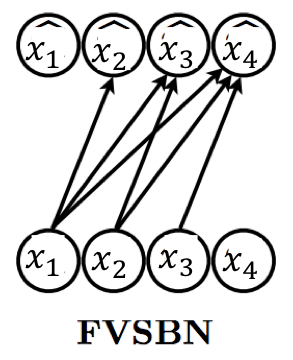
\includegraphics[height=1.0in]{images/arm/fvsbn.png}
    \caption{A fully visible sigmoid belief network over 4 variables}
\end{figure}

\framebreak

\begin{itemize}
    \setlength{\itemsep}{-0.25em}
    \item The conditional variables $X_i | X_1, X_2, \cdots X_{i-1}$ are Bernoulli with parameters
    \vspace{-1em}
    \begin{equation*}
        \hat{x}_i = \mathcal{P}(X_i=1 \mid x_1, \cdots, x_{i-1}; \alpha^i) = \mathcal{P}(X_i=1 \mid x_{<i}; \alpha^i) = \sigma (\alpha_0^i + \sum^{i-1}_{j=1}\alpha_j^i x_j)
    \end{equation*}
    \vspace{-1.5em}
    \item To evaluate $\mathcal{P}(x)$, we just multiply all the conditionals.
    \item To sample new images, we sample each $X_i$ chronologically.
    \begin{itemize}
        \item Sample $\overline{x}_1 \sim \mathcal{P}(x_1)$ np.random.choice([1,0], p=[$\hat{x}, 1-\hat{x}$])
        \item Sample $\overline{x}_2 \sim \mathcal{P}(x_2 | X_1=\overline{x}_1)$
        \item Sample $\overline{x}_3 \sim \mathcal{P}(x_3 | X_1=\overline{x}_1, X_2=\overline{x}_2)$
    \end{itemize}
    \item Total number of parameters = $1+2+3+ \cdots +n = \frac{n(n+1)}{2}$
    \item \textbf{Pros:} The likelihood is tractable and can be computed exactly.
    \item \textbf{Cons:} Poor scalability: each variable $x_i$ requires its own set of weights and bias, leading to a quadratic number of parameters as the number of variables increases.
\end{itemize}
\end{frame}


\begin{frame}{FVSBN: Results}

\begin{figure}
    \centering
    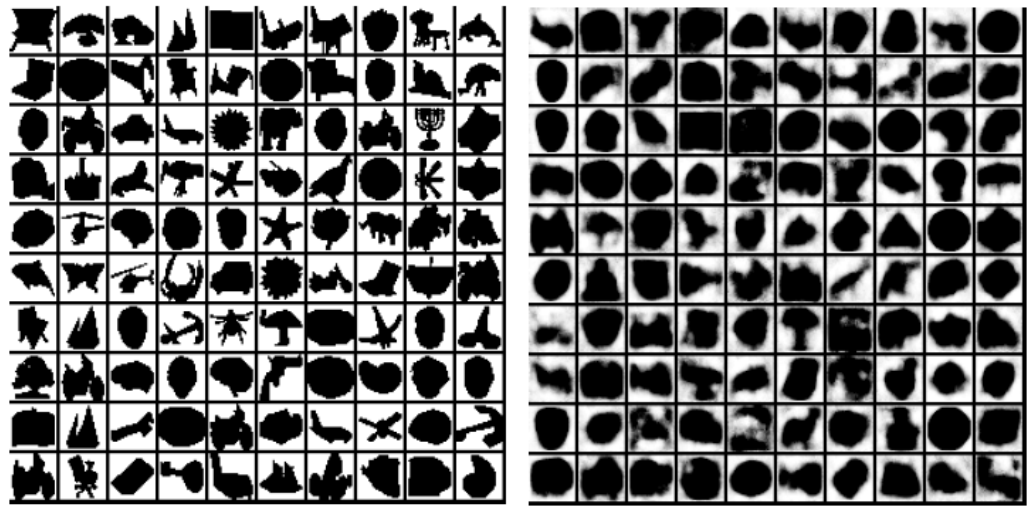
\includegraphics[height=2.0in]{images/arm/fvsbn_results.png}
    \caption{FVSBN results. Left: Training data. Right: Samples generated by model (Learning Deep Sigmoid Belief Networks with Data Augmentation, 2015)}
\end{figure}
    
\end{frame}
\begin{frame}[allowframebreaks]{Neural Autoregressive Density Estimation (NADE)}
\textbf{Introduced by:} Larochelle and Murray (2011)

\textbf{Goal:} Provide an efficient and scalable version of Fully Visible Sigmoid Belief Networks (FVSBN) by using shared weights and a feedforward neural network.

\textbf{Main Idea:}
\begin{itemize}
    \item Uses a masked neural network to estimate each conditional probability:
    \vspace{-0.5em}
    \begin{equation*}
        p(\mathbf{x}) = \prod_{i=1}^n p(x_i \mid x_{<i})
    \end{equation*}
    \vspace{-0.5em}
    \item Efficiently computes gradients via weight sharing and dynamic masking.
\end{itemize}

\textbf{Advantages:}
\begin{itemize}
    \item Tractable and scalable.
    \item Inspired later models such as MADE and normalizing flows.
\end{itemize}

\framebreak
\textbf{Model Structure:}
\begin{itemize}
    \item Each variable $x_i$ is modeled conditionally on all previous variables $x_{<i}$.
    \item Uses a neural network to compute the conditional probabilities.
    \item The weights are shared across different variables, reducing the number of parameters significantly.
\end{itemize}
\textbf{Formulation:}
\begin{itemize}
    \item The conditional probability is modeled as:
    \begin{equation*}
        p(x_i \mid x_{<i}) = \sigma(\alpha^{(i)} h_i + b_i)
    \end{equation*}
    where $h_i$ is a hidden representation computed from the previous variables, $\alpha^{(i)}$ are the weights, and $b_i$ is a bias term.
\end{itemize}
\textbf{Neural Network Layer:}

NADE uses a neural network layer instead of just logistic regression to improve model performance.
    $$h_i = \sigma(\mathbf{W}_{.,<i} x_{<i} + c)$$
    $$f_i(x_1,x_2,\cdots,x_{i-1}) = \sigma(\alpha^{(i)}h_i+b_i)$$

\begin{figure}
    \centering
    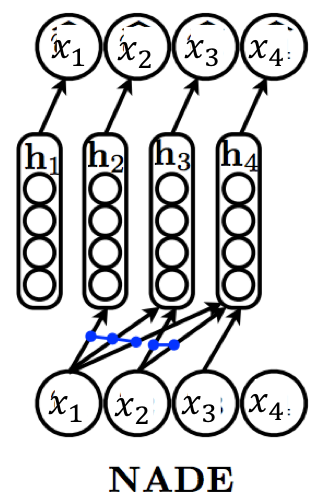
\includegraphics[height=1.0in]{images/arm/nade.png}
    \caption{A neural autoregressive density estimator over four variables. Blue connections donate shared weights.}
\end{figure}

\end{frame}

\begin{frame}{NADE Results}

\begin{figure}
    \centering
    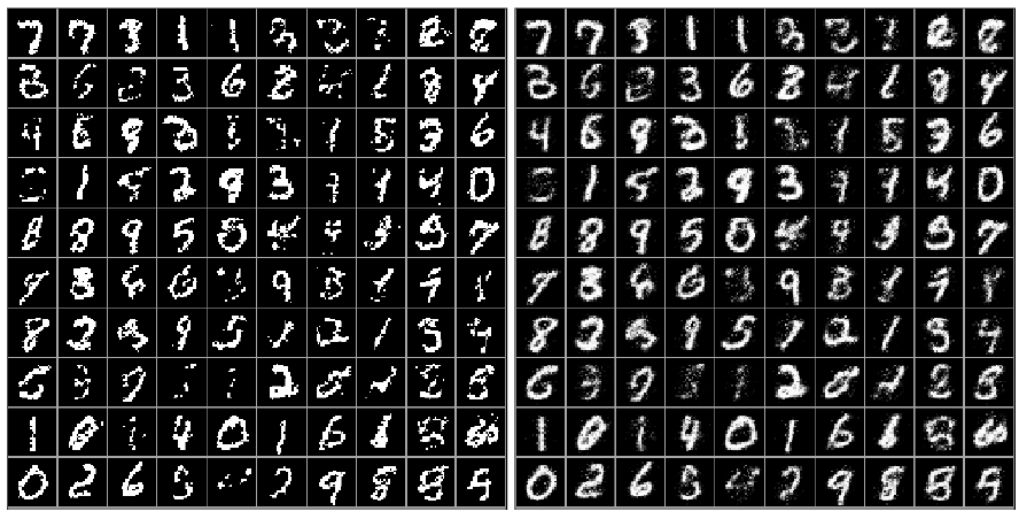
\includegraphics[height=2.0in]{images/arm/nade_results.png}
    \caption{NADE results. Left: Samples generated by model. Right: Conditional Probabilities $\hat{x}_i$ (The Neural Autoregressive Distribution Estimator, 2011)}
\end{figure}

\end{frame}

\begin{frame}{Non-Binary Outputs}
    \begin{itemize}
        \item What if the output variable is not binary? For example, we have to predict pixel value between 0 and 255.
        \item One solution: Let $\mathbf{\hat{x}}_i$ parameterize a categorical distribution
        \begin{align}
            h_i = \sigma(\mathbf{W}_{.,<i} x_{<i} + c)\\
            \mathcal{P}(x_i | x_1, \cdots, x_{i-1}) = \text{Cat}(p_i^1, \cdots, p_i^K)\\
            \mathbf{\hat{x}}_i = (p_i^1, \cdots, p_i^K) = \text{softmax} (A_i h_i + b_i)
        \end{align}
        \item Softmax generalizes the sigmoid function $\sigma(\cdot)$ and transforms a vector of K numbers into a vector of K probabilities (non-negative, sum to 1).

    \end{itemize}
\end{frame}

\begin{frame}[allowframebreaks]{RNADE – Real-valued NADE}
    \begin{itemize}
        \item How to model continuous random variables $X_i \in \mathbb{R}$?
        \item Solution: Let $\mathbf{\hat{x}}_i$ parameterize a continuous distribution.
        \item This was introduced in RNADE.
        \item $\mathbf{\hat{x}}_i$ defines the mean and stddev of Gaussian Random Variable $(\mu^j_i, \sigma^j_i)$
    \end{itemize}

    \framebreak

    \textbf{Introduced by:} Uria et al. (2013)

    \vspace{1em}
    RNADE (Real-valued Neural Autoregressive Density Estimator) extends NADE to handle continuous data.

    \begin{itemize}
        \item \textbf{Extension:} Uses a mixture of Gaussians for each conditional distribution.
        \item \textbf{Conditional Density:}
        \[
            p(x_i \mid x_{<i}) = \sum_{k=1}^K \pi_k \, \mathcal{N}(x_i \mid \mu_k, \sigma_k^2)
        \]
        \item The parameters of each mixture component (weights $\pi_k$, means $\mu_k$, variances $\sigma_k^2$) are produced by a neural network conditioned on $x_{<i}$.
    \end{itemize}

    \framebreak
    \textbf{Formulation:}
    \begin{itemize}
        \item The joint probability is factorized as:
        \[
            p(\mathbf{x}) = \prod_{i=1}^n p(x_i \mid x_{<i})
        \]
        \item Each conditional is modeled as:
        \[
            p(x_i \mid x_{<i}) = \sum_{k=1}^K \pi_k(x_{<i}) \, \mathcal{N}(x_i \mid \mu_k(x_{<i}), \sigma_k^2(x_{<i}))
        \]
        where $\pi_k$, $\mu_k$, and $\sigma_k$ are outputs of a neural network conditioned on $x_{<i}$.
    \end{itemize}

    \textbf{Applications:}
    \begin{itemize}
        \item Density estimation for real-valued data (e.g., audio, speech).
    \end{itemize}
    
    \framebreak
    \textbf{Pros:}
    \begin{itemize}
        \item Powerful for modeling complex continuous distributions.
        \item Influential precursor to more advanced autoregressive flows.
    \end{itemize}

    \textbf{Cons:}
    \begin{itemize}
        \item Still suffers from scalability issues with high-dimensional data.
        \item Requires careful tuning of the number of mixture components.
    \end{itemize}
\end{frame}
\begin{frame}[allowframebreaks]{Learning Autoregressive Models}
\begin{itemize}
    \item The goal of learning is to return a model $\hat{\mathcal{M}}$ that precisely captures the distribution $\mathcal{P}_{data}$ from which our data was sampled
    \item This is in general not achievable because of
    \begin{itemize}
        \item limited data only provides a rough approximation of the true underlying distribution
        \item computational reasons
    \end{itemize}
    \item Example. Suppose we represent each MNIST digit with a vector $\mathbf{X}$ of 784 binary variables (black vs. white pixel). How many possible states (= possible images) in the model? $2^{784} \approx 10^{236}$ . Even $10^7$ training examples provide extremely sparse coverage!
    \item We want to select $\hat{\mathcal{M}}$ to construct the ”best” approximation to the underlying distribution $\mathcal{P}_{data}$


\end{itemize}

\framebreak

\begin{itemize}
    \item We want to learn the full distribution so that later we can answer any probabilistic inference query
    \item We want to construct $\mathcal{P}_{\theta}$ as ”close” as possible to $\mathcal{P}_{data}$ (recall we assume we are given a dataset $\mathcal{D}$ of samples from $\mathcal{P}_{data}$)
    \begin{figure}
        \centering
        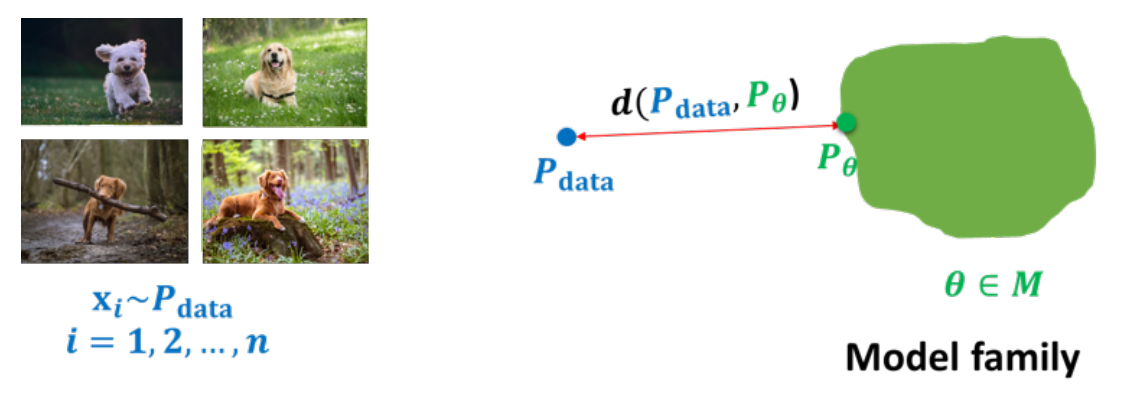
\includegraphics[height=1.3in]{images/autoregressive/learning.png}
        \caption*{Learning a generative model. $d(\cdot)$ is a distance measure.}
    \end{figure}
    
\end{itemize}
\end{frame}

\begin{frame}[allowframebreaks]{KL Divergence}
    \begin{itemize}
        \item How do we evaluate ”closeness” between model and data distribution?
        \item \textbf{Kullback-Leibler divergence} (KL-divergence) is one possibility:
        $$D(\mathcal{P}_{data}||\mathcal{P}_{\theta}) = E_{x \sim \mathcal{P}_{data}}   \left [log \left ( \frac{\mathcal{P}_{data}(x)}{\mathcal{P}_{\theta}(x)} \right ) \right ] = \sum_{x} \mathcal{P}_{data}(x) log \frac{\mathcal{P}_{data}(x)}{\mathcal{P}_{\theta}(x)}$$
        \item $D(\mathcal{P}_{data}||\mathcal{P}_{\theta})$ iff the two distributions are the same.
        \item It measures the ”compression loss” (in bits) of using $\mathcal{P}_{\theta}$ instead of $\mathcal{P}_{data}$.
    \end{itemize}
\end{frame}

\begin{frame}{Expected Log-Likelihood}

\begin{itemize}
    \item We can simplify this somewhat:
    \begin{equation}
    \begin{split}
        D(\mathcal{P}_{data}||\mathcal{P}_{\theta}) & = E_{x \sim \mathcal{P}_{data}}   \left [log \left ( \frac{\mathcal{P}_{data}(x)}{\mathcal{P}_{\theta}(x)} \right ) \right ] \\
         & = E_{x \sim \mathcal{P}_{data}} [log \mathcal{P}_{data}(x)] - E_{x \sim \mathcal{P}_{data}} [log \mathcal{P}_{\theta}(x)]
    \end{split}
    \end{equation}
    
    \item The first term does not depend on $\mathcal{P}_{\theta}$. Then, \emph{minimizing} KL divergence is equivalent to \emph{maximizing} the \textbf{expected log-likelihood}
    \begin{equation}
    \begin{split}
        \arg\min_{\mathcal{P}_{\theta}} D(\mathcal{P}_{data}||\mathcal{P}_{\theta}) & = \arg\min_{\mathcal{P}_{\theta}} - E_{x \sim \mathcal{P}_{data}} [log \mathcal{P}_{\theta}(x)]\\
        & = \arg\max_{\mathcal{P}_{\theta}} E_{x \sim \mathcal{P}_{data}} [log \mathcal{P}_{\theta}(x)]
    \end{split}
    \end{equation}
    
    \begin{itemize}
        \item Asks that $\mathcal{P}_{\theta}$ assign high probability to instances sampled from $\mathcal{P}_{data}$, so as to reflect the true distribution
        \item Because of log, samples $x$ where $\mathcal{P}_{\theta}(x) \approx 0$ weigh heavily in objective

    \end{itemize}
    \item Although we can now compare models, since we are ignoring $H(\mathcal{P}_{data})$, we don’t know how close we are to the optimum.
    \item Problem: In general we do not know $\mathcal{P}_{data}$

\end{itemize}
\end{frame}

\begin{frame}{Maximum Likelihood}
\begin{itemize}
    \item Approximate the expected log-likelihood
    $$ E_{x \sim \mathcal{P}_{data}} [log \mathcal{P}_{\theta}(x)]$$
    with the empirical log-likelihood:
    $$E_{\mathcal{D}} = \frac{1}{\mathcal{D}} \sum_{x \in \mathcal{D}} log \mathcal{P}_{\theta}(x)$$
    \item \textbf{Maximum likelihood learning} is then:
        $$\arg\max_{\mathcal{P}_{\theta}} \frac{1}{\mathcal{D}} \sum_{x \in \mathcal{D}} log \mathcal{P}_{\theta}(x)$$
\end{itemize}
\end{frame}

\begin{frame}[allowframebreaks]{Recurrent Neural Networks (RNN)}
\begin{itemize}
    \item The next form of autoregressive models
    \item \textbf{Challenge}: model $\mathcal{P}(x_t|x_{1:t-1}; \alpha^t)$. "History" $x_{1:t-1}$ keeps getting longer.
    \item \textbf{Idea}:  keep a summary and recursively update it
    \end{itemize}
    % \begin{figure}
    %     \centering
    %     \includegraphics[height=1.3in]{./images/rnn.PNG}
    %     \caption*{Recurrent Neural Network (RNN) samaple architecture.}
    % \end{figure}
    % \item Hidden layer $h_t$ is a summary of the inputs seen till time $t$

\framebreak
\begin{figure}
    \centering
    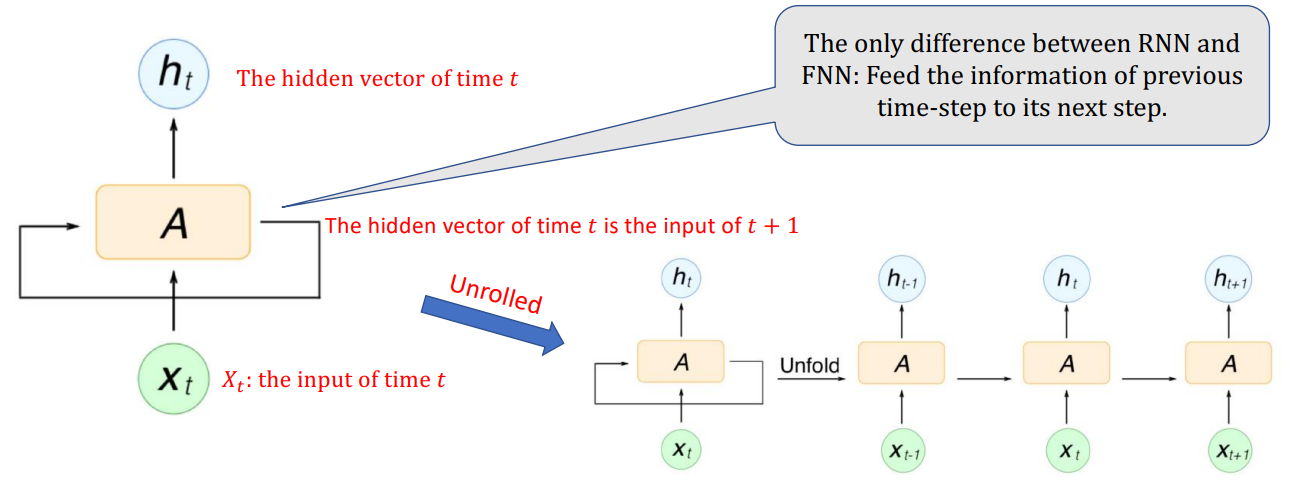
\includegraphics[height=0.9\textheight, width=\textwidth, keepaspectratio]{images/autoregressive/rnn_2.png}
    \caption*{Recurrent Neural Network (RNN) sample architecture.}
\end{figure}

\framebreak
Pros:
\begin{itemize}
    \item Can be applied to sequences of arbitrary length.
    \item Very general: For every computable function, there exists a finite RNN that can compute it
\end{itemize}
\vskip 10pt
Cons:
\begin{itemize}
    \item Still requires an ordering
    \item Sequential likelihood evaluation (very slow for training)
    \item Sequential generation (unavoidable in an autoregressive model)
    \item Can be difficult to train (vanishing/exploding gradients)
\end{itemize}
\end{frame}

\begin{frame}{RNNs}

\framebreak
\begin{figure}
    \centering
    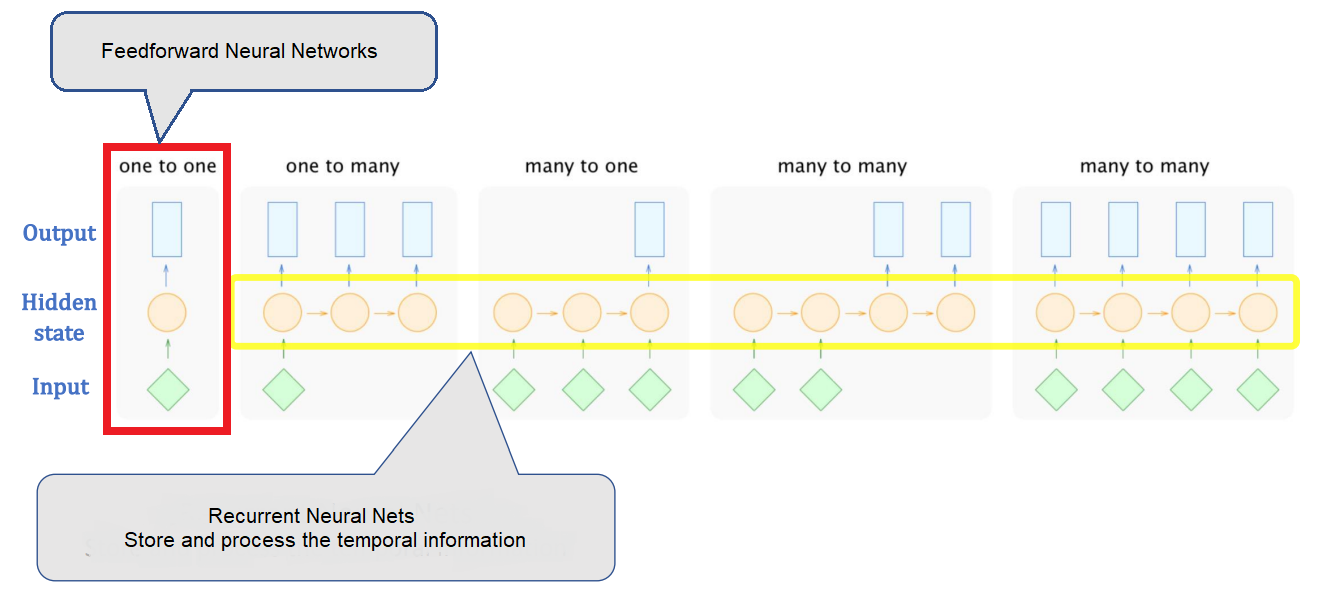
\includegraphics[height=0.9\textheight, width=\textwidth, keepaspectratio]{images/autoregressive/rnn_types.png}
    \caption*{Different sequential modeling types}
\end{figure}
    
\end{frame}

\begin{frame}[allowframebreaks]{RNNs - Examples}
\textbf{Image Captioning}
\begin{figure}
    \centering
    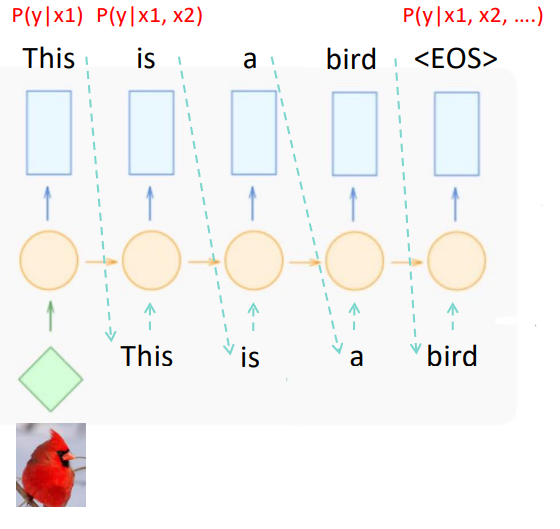
\includegraphics[height=0.7\textheight, width=\textwidth, keepaspectratio]{images/autoregressive/image_cap.png}
    \caption*{Image captioning with RNNs}
\end{figure}

\framebreak
\textbf{Text Generation}
\begin{figure}
    \centering
    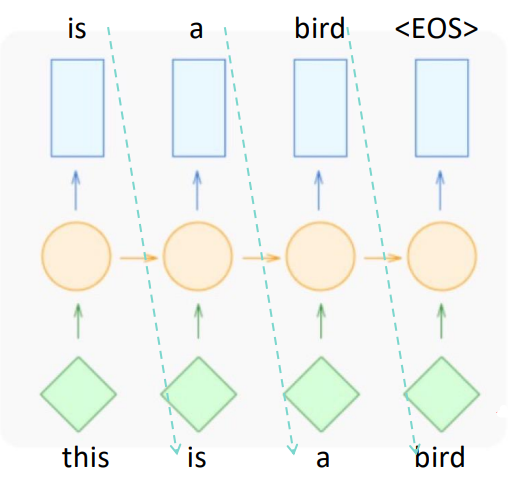
\includegraphics[height=0.7\textheight, width=\textwidth, keepaspectratio]{images/autoregressive/text_gen_ex.png}
    \caption*{Text generation with RNNs}
\end{figure}

\framebreak
\textbf{Chatbot}
\begin{figure}
    \centering
    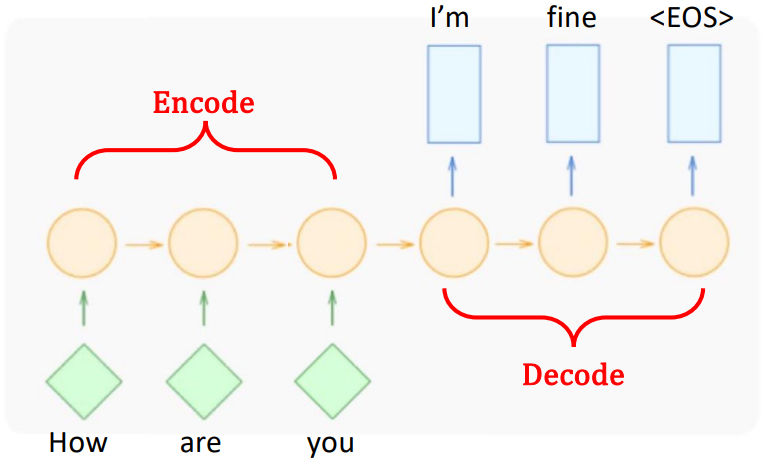
\includegraphics[height=0.7\textheight, width=\textwidth, keepaspectratio]{images/autoregressive/chatbot.png}
    \caption*{Chatbot with RNNs}
\end{figure}
\end{frame}
\begin{frame}[allowframebreaks]{PixelRNN – Pixel Recurrent Neural Network}
    \textbf{Introduced by:} van den Oord et al. (2016)

    \vspace{1em}
    \textbf{What is PixelRNN?}

    \begin{itemize}
        \item PixelRNN is a generative model specifically designed for image generation.
        \item It models the joint distribution of all pixels in an image by predicting one pixel at a time.
        \item Pixels are generated in a raster-scan order (left to right, top to bottom).
        \item Uses an autoregressive approach, where each pixel is generated conditioned on all previously generated pixels.
    \end{itemize}  

    \framebreak
    
    \textbf{Core Idea:}
    The model factorizes the image distribution as:
    \[
    p(\mathbf{x}) = \prod_{i=1}^{n} p(x_i \mid x_1, x_2, \ldots, x_{i-1})
    \]
    where each pixel $x_i$ is conditioned on all previous pixels $(x_1, x_2, \ldots, x_{i-1})$.

    Each pixel's value (such as its RGB channels) is predicted based on all preceding pixels using a recurrent neural network, allowing the model to capture complex dependencies and structures within the image.
    
    \framebreak
    \textbf{Architecture of PixelRNN}

    \begin{enumerate}
        \setlength{\itemsep}{-0.25em}
        \item \textbf{Input Representation:}
        \begin{itemize}
            \setlength{\itemsep}{-0.25em}
            \item Each image is a 2D grid of pixels.
            \item Each pixel can have multiple channels (e.g., RGB).
        \end{itemize}

        \item \textbf{Autoregressive Modeling:}
        \begin{itemize}
            \item For each pixel, the model learns $p(x_{i,j} \mid x_{<i,j})$, where $x_{<i,j}$ are all pixels above and to the left of the current pixel $(i, j)$.
        \end{itemize}

        \item \textbf{RNN Layers:}
        \begin{itemize}
            \item Uses RNNs along the rows of the image:
            \begin{itemize}
                \item \textbf{Row LSTM:} Processes one row at a time from left to right.
                \item \textbf{Diagonal BiLSTM:} Processes diagonals in the image to improve context.
            \end{itemize}
        \end{itemize}

        \item \textbf{Masked Convolutions:}
        \begin{itemize}
            \item Prevent the model from “seeing the future” pixels.
            \item Each convolution is masked to preserve the autoregressive property.
        \end{itemize}
    \end{enumerate}

    \framebreak
    \begin{figure}
        \centering
        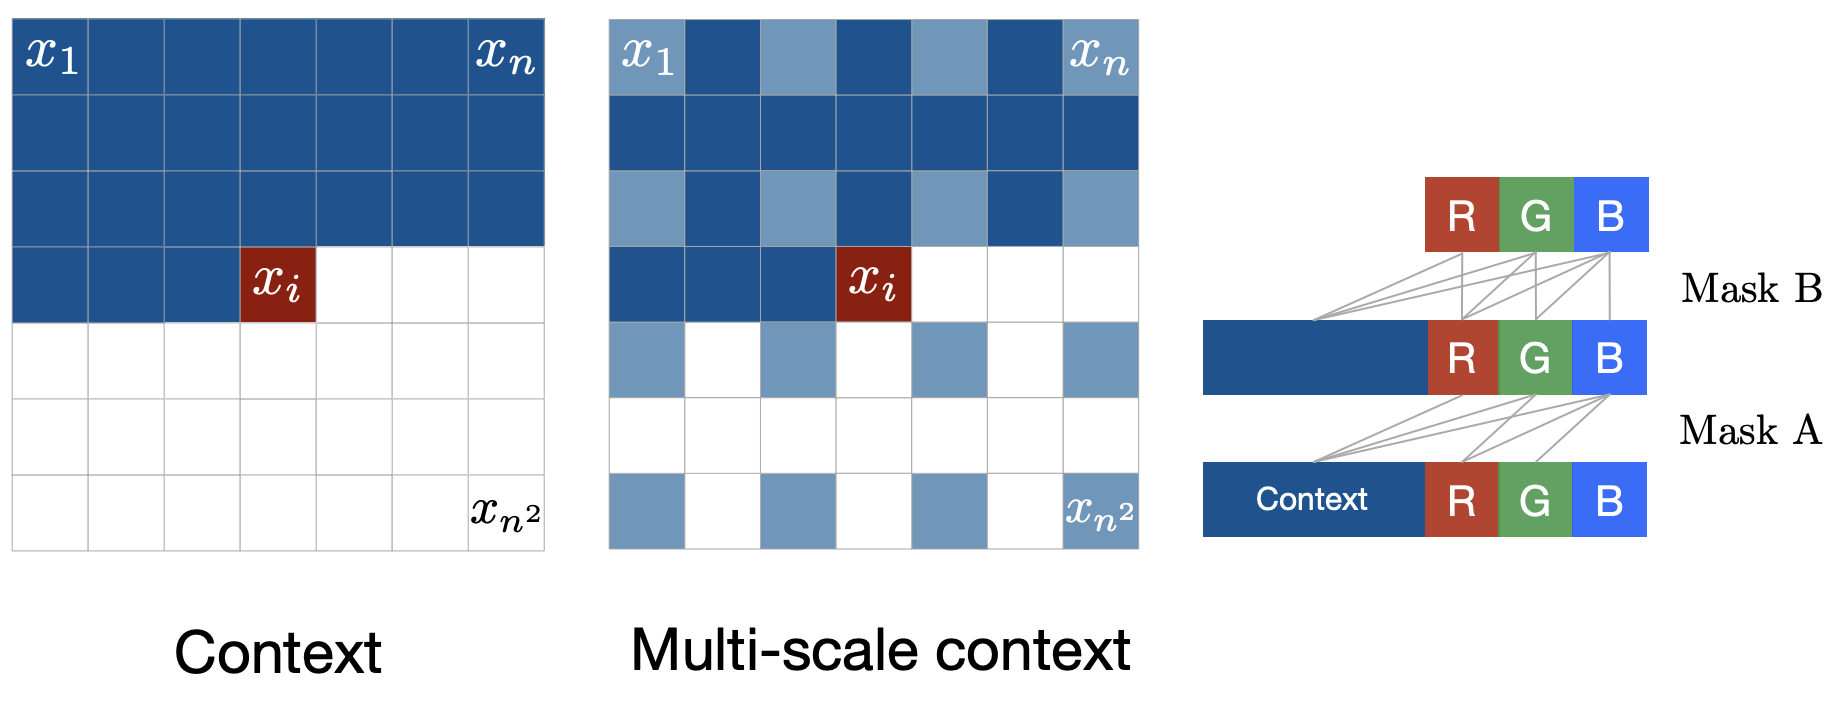
\includegraphics[height=1.0in]{images/arm/pixel-rnn.png}
        \caption{Left: To generate pixel xi one conditions on all the previously generated pixels left and above of xi. Center: To generate a pixel in the multi-scale case we can also condition on the
subsampled image pixels (in light blue). Right: Diagram of the
connectivity inside a masked convolution. In the first layer, each
of the RGB channels is connected to previous channels and to the
context, but is not connected to itself. In subsequent layers, the
channels are also connected to themselves.}
    \end{figure}

    \framebreak

    \begin{columns}
        \begin{column}{0.4\textwidth}
            \textbf{Types of RNNs in PixelRNN}

            \begin{itemize}
                \item \textbf{Row LSTM:}
                \begin{itemize}
                    \item Applies a 1D LSTM across each row.
                    \item Information flows left-to-right in each row.
                    \item Maintains the autoregressive structure.
                \end{itemize}

                \item \textbf{Diagonal BiLSTM:}
                \begin{itemize}
                    \item Applies a 2D LSTM diagonally across the image.
                    \item Allows pixels to be conditioned on a broader context.
                \end{itemize}
            \end{itemize}
        \end{column}
        \begin{column}{0.6\textwidth}
            \begin{figure}
                \centering
                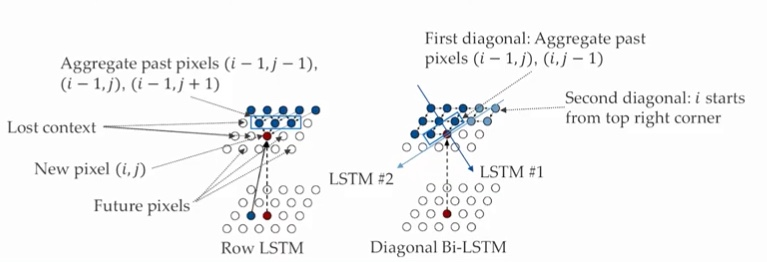
\includegraphics[width=1.1\textwidth,keepaspectratio]{images/arm/pixel-rnn-networks.png}
                \caption{PixelRNN architecture with Row LSTM and Diagonal BiLSTM. The model processes pixels in a raster-scan order, ensuring that each pixel is conditioned on all previously generated pixels.}
            \end{figure}
        \end{column}
    \end{columns}

    \framebreak
    \textbf{Training and Inference:}
    \begin{itemize}
        \item \textbf{Training:} The model is trained using maximum likelihood estimation (MLE) to maximize the joint probability of the pixels in the training images.
        \item \textbf{Inference:} During inference, pixels are generated sequentially, starting from a blank canvas and conditioning each new pixel on all previously generated pixels.
        \item \textbf{Sampling:} The model can sample new images by repeatedly predicting the next pixel based on the current image context.
    \end{itemize}

    \begin{figure}
        \centering
        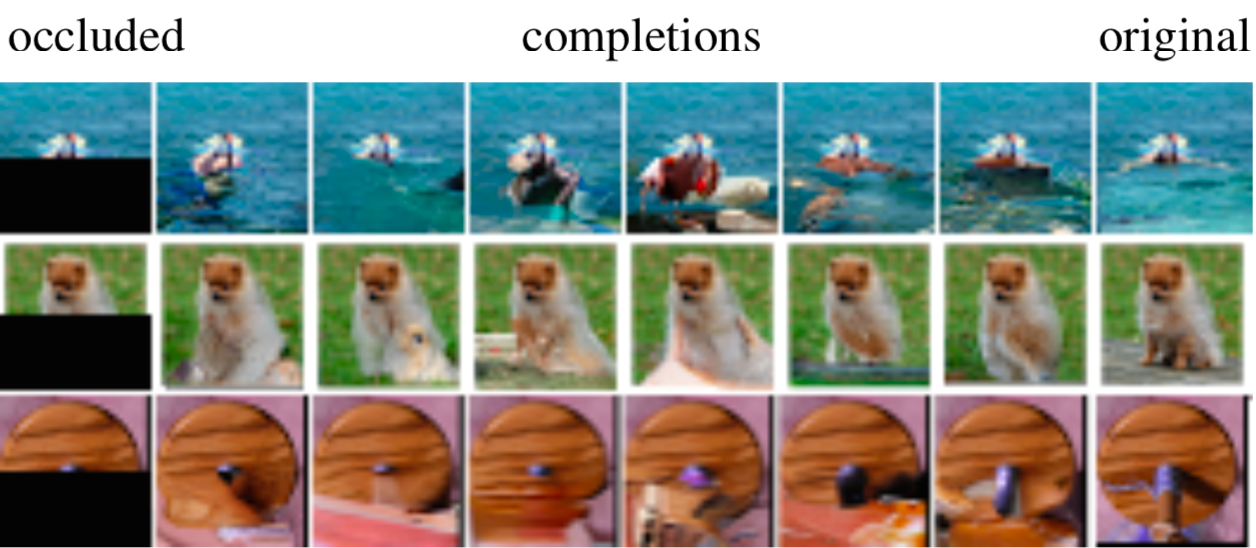
\includegraphics[width=\textwidth,keepaspectratio]{images/arm/example-pixel-rnn.png}
        \caption{Image completions sampled from a PixelRNN.}
    \end{figure}

    \framebreak
    \textbf{Pros:}
    \begin{itemize}
        \item Capable of generating high-quality images with complex structures.
        \item Effective at capturing long-range dependencies in images.
    \end{itemize}

    \textbf{Cons:}
    \begin{itemize}
        \item Computationally intensive due to sequential processing of pixels.
        \item Slower inference compared to parallelizable models like PixelCNN.
    \end{itemize}
\end{frame}